\section{Entwicklung zur DevOps-Kultur} \label{entwicklung}
Es ist denkbar, einen gewissen Teil von Continuous Delivery auch ohne DevOps einzuführen, denn hierfür muss es nicht zwingendermaßen gemischte Teams geben, sondern lediglich eine Zusammenarbeit an der Continuous-Delivery-Pipeline. Continuous Delivery verfolgt unterschiedliche Ziele von denen einige trotz einer reduzierten Pipeline erreicht werden können, ohne, dass eine völlige Umorganisation notwendig ist.
Letztendlich bringen diese Ansätze allerdings weniger Vorteile mit sich. Wenn Continuous Delivery vollständig umgesetzt werden soll, gelingt dies nur mit der Einführung von DevOps. DevOps einzuführen, bedeutet jedoch eine fundamentale Änderung der Organisation. Eine solche Änderung ist mit einem erheblichen Aufwand verbunden und kann vor allem in großen Konzernen schwer umsetzbar sein. In diesem Kapitel wird darauf eingegangen, welche Aspekte dabei zu berücksichtigen sind und welche Folgen diese Transformation für Unternehmen hat [1].

\subsection{Umsetzung von Continuous Delivery}
Continuous Delivery ist vor allem eine technische Praktik. Trotzdem hat diese Disziplin verschiedene Auswirkungen auf die Organisation. Continuous Delivery steht und fällt mit der Pipeline. Das Umsetzen einer einfachen Delivery-Pipeline kann bereits mit simplen mitteln erfolgen. Vor allem zu Beginn eines Projekts kann der Aufbau einer solchen Pipeline verfolgt werden. Beispielsweise kann ein Unternehmen hier vorab mit den Phasen Commit und Deploy beginnen, da diese schließlich existieren müssen. Es ist dann möglich, die Pipeline im weiteren Verlauf schrittweise weiterzuentwickeln, indem entsprechende Phasen (z. B. automatisierte Tests) hinzugefügt werden. Wird Continuous Delivery zum Start eines Projekts eingeführt, kann dies auch bei der Auswahl der Technologien und Architekturen berücksichtigt werden [1]. \\ \\
Oft setzt Continuous Delivery allerdings an eine bestehende Codebasis an, die nicht dafür konzipiert wurde. In gewisser Weise besteht immer eine Delivery-Pipeline, da es stets einen Prozess zur Auslieferung der Software gibt. Nur kann dieser Prozess sehr komplex sein. Das Ziel von Continuous Delivery ist allerdings einen konstanten Fluss von Features und Codeänderungen durch die Pipeline zu erreichen. Um die bestehende Pipeline entsprechend anzupassen können verschiedene Ansätze wie beispielsweise Value Stream Mapping angewandt werden. Aus dieser Analysetechnik lassen sich dann Optimierungen ableiten. Zu weiteren Optimierungsmaßnahmen gehört auch DevOps [1]. Value Stream Mapping hingegen wird in dieser Arbeit nicht weiter beleuchtet. \\ \\
Beim Übernehmen von Continupus Delivery reicht es allerdings oft nicht, schlicht entsprechende Werkzeuge zu verwenden. Solange die Prozesse innerhalb der Organisation nicht ablaufen, wie bei einer gut geölten Maschine, kann hier keine signifikante Steigerung der Effizienz erreicht werden [5]. Der Schlüssel, um entsprechende Prozesse gut zum Laufen zu bringen ist dabei DevOps. Mit dieser Organisationsform funktioniert Continuous Delivery besonders gut, da hierfür das Wissen aus beiden Abteilungen benötigt wird. Während die Entwicklung die Anwendung, deren Konfiguration und Aufbau kennt, weiß der Betrieb über die Rahmenbedingungen bescheid [1].


\subsection{Umsetzung von DevOps}
Continuous Delivery ist hauptsächlich mit der DevOps-Bewegung verbunden [3], da DevOps eine wirkungsvolle Optimierungsmaßnahme darstellt. Dabei fokussiert sich dieser Ansatz auf die Liefergeschwindigkeit, das kontinuierliche Testen in Produktionsähnlichen Umgebungen, kontinuierliche Rückmeldung und schnelle Reaktionsfähigkeit sowie, wie der Name bereits andeutet, das Auflösen der Teamgrenzen [5]. Immerhin sollen die Entwicklung und der Betrieb als eine Einheit agieren und Teams anhand von Komponente oder fachlichen Zuständigkeiten aufgeteilt werden, wodurch auch die vollständige Verantwortung für ein Modul bei dem entsprechenden Team liegt. Damit geht eine Änderung der Organisationsform einher, um eine Kultur und ein Umfeld zu schaffen, indem das Erstellen, Testen und Freigeben von Software schnell, häufig und zuverlässig erfolgen kann. Ein Großteil von DevOps befasst sich demnach mit der Prozessverbesserung durch eine radikale Automatisierung manueller Prozesse [7]. \\ \\
Viele Unternehmen sind bereits dabei, DevOps erfolgreich umzusetzen. Allerdings bleiben nach wie vor kritische Barrieren bei der Entwicklung, wie sie im folgenden Kapitel näher beschrieben werden. Um diese Philosophie anzuwenden gibt es verschiedene Möglichkeiten. Dabei ist vermutlich die größte Hürde die Angst vor Veränderungen (siehe vorherige Abneigung gegenüber Clouds) [3]. \\ \\
Es muss einem klar sein, was DevOps für das Unternehmen bedeutet. Zwei der größten Hindernisse, diese Disziplin erfolgreich umzusetzen, sind die Unternehmensarchitektur sowie Unternehmenskultur, die davon beeinflusst werden.


\subsection{Architektur}
Für die Architektur bedeutet DevOps eine Herausforderung. Da eine zentrale Instanz, die die Architektur in eine bestimmte Richtung zwingt einen Widerspruch zu den selbständigen Teams darstellt, müssen an dieser Stelle Abstimmungen erfolgen. Die Teams entwickeln so die Architektur des Systems untereinander. Die Erfahrung hat gezeigt, dass entsprechend moderierte Meetings stattfinden, in welchen die Teams ihre Abstimmung vornehmen können [1].\\ \\
Continuious Delivery und DevOps sind Ansätze, mit denen Software effizienter und effektiver betrieben und in Produktion gebracht werden kann. Sie haben vor allem Auswirkungen auf Deployment- und Betriebsprozesse. Allerdings beeinflusst Continuous Delivery auch die Architektur der Lösungen. Wenn bei einem System an einer Stelle etwas geändert wird, muss die ganze Pipeline durchlaufen werden. Es werden dabei nicht nur die geänderten Komponenten getestet, sondern alle. Das führt zu einer Menge unnötiger Arbeit und verzögert das Feedback. Bis zu einem gewissen Maße ist dies sinnvoll, da beim Durchlaufen der Pipeline alle Bestandteile getestet werden sollen. Immerhin kann sich ein Fehler in einer Komponente erst dadurch manifestieren, wenn eine abhängige Komponente ein falsches Verhalten aufweist [1].\\ \\
Durch Continuous Delivery ergibt sich eine andere technische Umsetzung der Komponenten, denn jede Komponente kann als eine eigene Deployment-Einheit implementiert werden, welche dann jeweils eine eigene Pipeline durchlaufen. Es wird demnach auch nicht mehr das gesamte System deployt, sondern nur ein Teil. Das schnelle Feedback und die in angestrebte Risikominimierung wird hierdurch erreicht. Es werden nun also zwei Merkmalen der Unternehmensarchitektur eine hohe Priorisierung zuteil: Testbarkeit und Einsatzfähigkeit. Das Design für die Implementierung und die entsprechenden Tests beginnt zudem mit der Sicherstellung, dass die Services aus lose gekoppelten, gut gekapselten Komponenten oder Modulen bestehen (im Rahmen der objektorientierten Programmierung folgen solche Systeme den Prinzipien des SOLID-Designs). Durch verschiedene Anpassungen der Architektur und den bisher erwähnten Anforderungen an die Organisation ergibt sich ein umfangreiches Zusammenwirken von Continuous Delivery und dem Softwarearchitekturansatz von Microservices. Microservices entsprechen sehr gut den Anforderungen an einer Architektur für ein Continuous Delivery System und setzen auch andere Aspekte (Technologiefreiheit, unabhängige Einheiten etc.) um [1]. Die Microservices-Bewegung hat diese architektonischen Eigenschaften sogar explizit priorisiert. Müssen beispielsweise viele Microservices gleichzeitig freigegeben werden („Big Bang-Event“), ist es erforderlich, dass viele Teams in einer sorgfältigen Art und Weise zusammenarbeiten. Solche Bereitstellungen können dabei typischerweise viele Stunden oder sogar Tage in Anspruch nehmen und erfordern eine erhebliche Planung. Auch hier ist die Verbindung zu DevOps wieder erkennbar. Ein Unternehmen muss kontinuierlich und vor allem agil planen. Das setzt voraus, dass es in der Lage ist, sich schnell an die sich ändernden Marktbedingungen anzupassen [3]. Bei der Einführung von Continuous Delivery muss also auch die Architektur der Software angepasst werden. Lediglich die Prozesse anzupassen bzw. zu ändern, reicht nicht aus [1].

\subsection{Kultur}
Auch die Unternehmenskultur ist von der Transformation betroffen. Obwohl diese nicht greifbar und nur schwer zu ändern ist, ist es wichtig, eine Kultur zu schaffen, in welcher alle Menschen der Organisation bei der Verfolgung gemeinsamer Ziele zusammenarbeiten. Dies ging bereits durch den Soziologen Ron Westrum hervor (…), der die Wichtigkeit einer solchen Kultur betonte. Bei DevOps wird immer die primäre Bedeutung der Kultur hervorgehoben, mit besonderem Fokus auf einer effektiven Zusammenarbeit zwischen Entwicklungsteams und IT-Betriebsteams. Tatsächlich warten die leistungsstärksten Unternehmen nicht darauf, dass schlimme Dinge passieren, um daraus zu lernen und sich zu verbessern. Sie schaffen regelmäßig (kontrollierte) Unfälle, um schneller Optimierungen abzuleiten und schneller als die Konkurrenz zu lernen [3]. Leistungsstarke Organisationen versuchen also stets besser zu werden. Durch die Eigenverantwortung und Selbstorganisation, um die es bei DevOps im Grunde geht, übernehmen die Teams die vollständige Verantwortung für ihre Komponenten. Dies Betrifft sowohl den Betrieb als auch die Entwicklung. Somit können viele Entscheidungen direkt in den Teams gefällt werden. Eine dieser Entscheidungen betrifft den zu verwendenden Technologie-Stack des Teams.

\subsection{Technolgie}
Die Technologiefreiheit bedeutet, dass die vollständige Zuständigkeit der Auswahl von Implementierungstechnologien wie Frameworks, Programmiersprachen oder Application Server bei den Teams liegt. Treten mit den ausgewählten Technologien Probleme auf, muss sich auch nur dieses Team mit der Behebung möglicher Fehler auseinandersetzen. Andere Teams bleiben davon unbeeinflusst. So können sehr viele unterschiedliche Technologien in einer Organisation genutzt werden. Eine klassische Organisation versucht, die Anzahl von Technologien möglichst einzuschränken und zu kontrollieren, um so Risiken zu minimieren und ein Zusammenspiel zu realisieren. Wenn alle Projekte dieselben Programmiersprachen und Infrastrukturelemente nutzen, kennt jeder Entwickler die notwendigen Technologien und kann jedes Projekt bis zu einem gewissen Maße unterstützen. Der Betrieb kann sich somit auch auf diese Technologien fokussieren und ist mit Problemen dieses Stacks besonders gut vertraut. Bei DevOps stehen Synergien nicht so sehr im Vordergrund. Der Fokus liegt auf der Freiheit der Teams, eigene Entscheidungen zu treffen. Dadurch kann jedes Team den Technologie-Stack wählen, der für die jeweiligen Herausforderungen am besten geeignet ist. Auf diese Weise kann jedes Team mit optimaler Produktivität arbeiten. Einen Standard-Technologie-Stack kann etabliert werden, indem auf Erfahrungen anderer Teams zurückgegriffen wird. Somit könnte es bereits einen Werkzeugkasten geben, welcher auch für andere Teams attraktiv ist [1].


%\begin{figure}[h!]
%	\centering
%	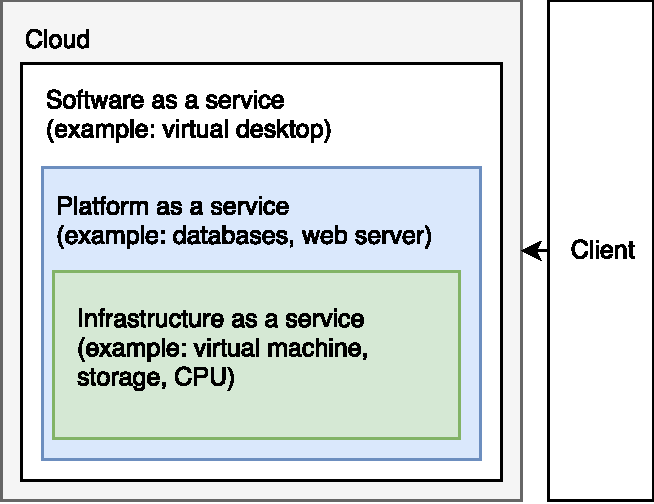
\includegraphics[width=0.8\linewidth]{images/servicemodules.pdf}
%	\caption{Cloud-Servicemodelle} %Generelle
%	\label{fig:cnn_structure}
%\end{figure}